%%%%%%%%%%%%%%%%%%%%%%%%%%%%%%%%%%%%%%%%%
% Jacobs Landscape Poster
% LaTeX Template
% Version 1.0 (29/03/13)
%
% Created by:
% Computational Physics and Biophysics Group, Jacobs University
% https://teamwork.jacobs-university.de:8443/confluence/display/CoPandBiG/LaTeX+Poster
% 
% Further modified by:
% Nathaniel Johnston (nathaniel@njohnston.ca)
%
% This template has been downloaded from:
% http://www.LaTeXTemplates.com
%
% License:
% CC BY-NC-SA 3.0 (http://creativecommons.org/licenses/by-nc-sa/3.0/)
%
%%%%%%%%%%%%%%%%%%%%%%%%%%%%%%%%%%%%%%%%%

%----------------------------------------------------------------------------------------
%	PACKAGES AND OTHER DOCUMENT CONFIGURATIONS
%----------------------------------------------------------------------------------------

\documentclass[final]{beamer}


\usefonttheme{serif} % default family is serif

\usepackage[utf8]{inputenc}
\usepackage[spanish]{babel} % for accented letters

\usepackage[none]{hyphenat} % stop the hyphenation

\usepackage{wrapfig} % for wrapping text around figures

\usepackage[scale=1.24]{beamerposter} % Use the beamerposter package for laying out the poster

\usepackage{longtable}

\usetheme{confposter} % Use the confposter theme supplied with this template

\setbeamercolor{block title}{fg=black,bg=white} % Colors of the block titles
\setbeamercolor{block body}{fg=black,bg=white} % Colors of the body of blocks
\setbeamercolor{block alerted title}{fg=white,bg=dblue!70} % Colors of the highlighted block titles
\setbeamercolor{block alerted body}{fg=black,bg=dblue!10} % Colors of the body of highlighted blocks
% Many more colors are available for use in beamerthemeconfposter.sty

%-----------------------------------------------------------
% Define the column widths and overall poster size
% To set effective sepwid, onecolwid and twocolwid values, first choose how many columns you want and how much separation you want between columns
% In this template, the separation width chosen is 0.024 of the paper width and a 4-column layout
% onecolwid should therefore be (1-(# of columns+1)*sepwid)/# of columns e.g. (1-(4+1)*0.024)/4 = 0.22
% Set twocolwid to be (2*onecolwid)+sepwid = 0.464
% Set threecolwid to be (3*onecolwid)+2*sepwid = 0.708

\newlength{\sepwid}
\newlength{\onecolwid}
\newlength{\twocolwid}
\newlength{\threecolwid}
\setlength{\paperwidth}{48in} % A0 width: 46.8in
\setlength{\paperheight}{36in} % A0 height: 33.1in
\setlength{\sepwid}{0.024\paperwidth} % Separation width (white space) between columns
\setlength{\onecolwid}{0.22\paperwidth} % Width of one column
\setlength{\twocolwid}{0.464\paperwidth} % Width of two columns
\setlength{\threecolwid}{0.708\paperwidth} % Width of three columns
\setlength{\topmargin}{-0.5in} % Reduce the top margin size
%-----------------------------------------------------------

\usepackage{graphicx}  % Required for including images

\usepackage{booktabs} % Top and bottom rules for tables

%----------------------------------------------------------------------------------------
%	TITLE SECTION 
%----------------------------------------------------------------------------------------

\title{New strategies for multi-factoral and temporal behavioral analyses} % Poster title


\author{Rayna M. Harris*\textsuperscript{1},
Suzanne H. Austin*\textsuperscript{2},
Andrew Lang\textsuperscript{3},
Matthew MacManes\textsuperscript{3},
Rebecca M. Calisi\textsuperscript{1}
} % Author(s)

\institute{*co-first authors, 1. University of California, Davis, 2. Oregon State University, 3. University of New Hampshire } % Institution(s)

%----------------------------------------------------------------------------------------

\begin{document}

\addtobeamertemplate{block end}{}{\vspace*{2ex}} % White space under blocks
\addtobeamertemplate{block alerted end}{}{\vspace*{2ex}} % White space under highlighted (alert) blocks

\setlength{\belowcaptionskip}{2ex} % White space under figures
\setlength\belowdisplayshortskip{2ex} % White space under equations

\begin{frame}[t] % The whole poster is enclosed in one beamer frame

\begin{columns}[t] % The whole poster consists of three major columns, the second of which is split into two columns twice - the [t] option aligns each column's content to the top

\begin{column}{\sepwid}\end{column} % Empty spacer column

\begin{column}{\onecolwid} % The first column



%----------------------------------------------------------------------------------------
%	INTRODUCTION
%----------------------------------------------------------------------------------------

\vspace{-0.5em}

\begin{block}{The problem}

Many differential genes expression profiling tools are designed to analyze simplistic experimental designs comparing treatment and control. However, experimental designs in behavioral neuroendocrinology often require many treatment groups to hone in on the causes and consequences of animal behavior. 

%\vspace{1em}


\end{block}


\begin{block}{\textit{Case study:} How and why do biological systems change over the course of parental care?}



\begin{figure}
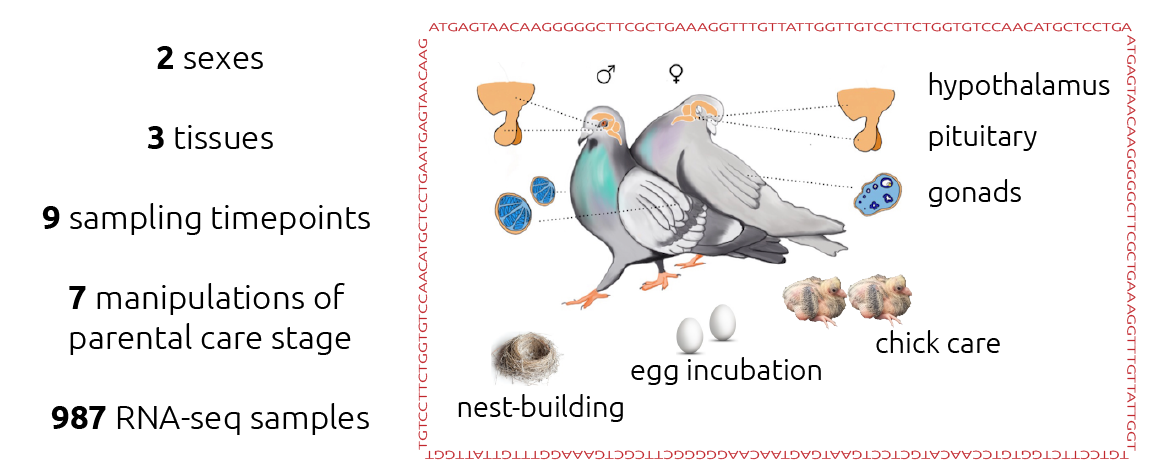
\includegraphics[width=0.9\linewidth]{DoveParentsRNAseq_approach-3.png}
\end{figure}


\begin{figure}
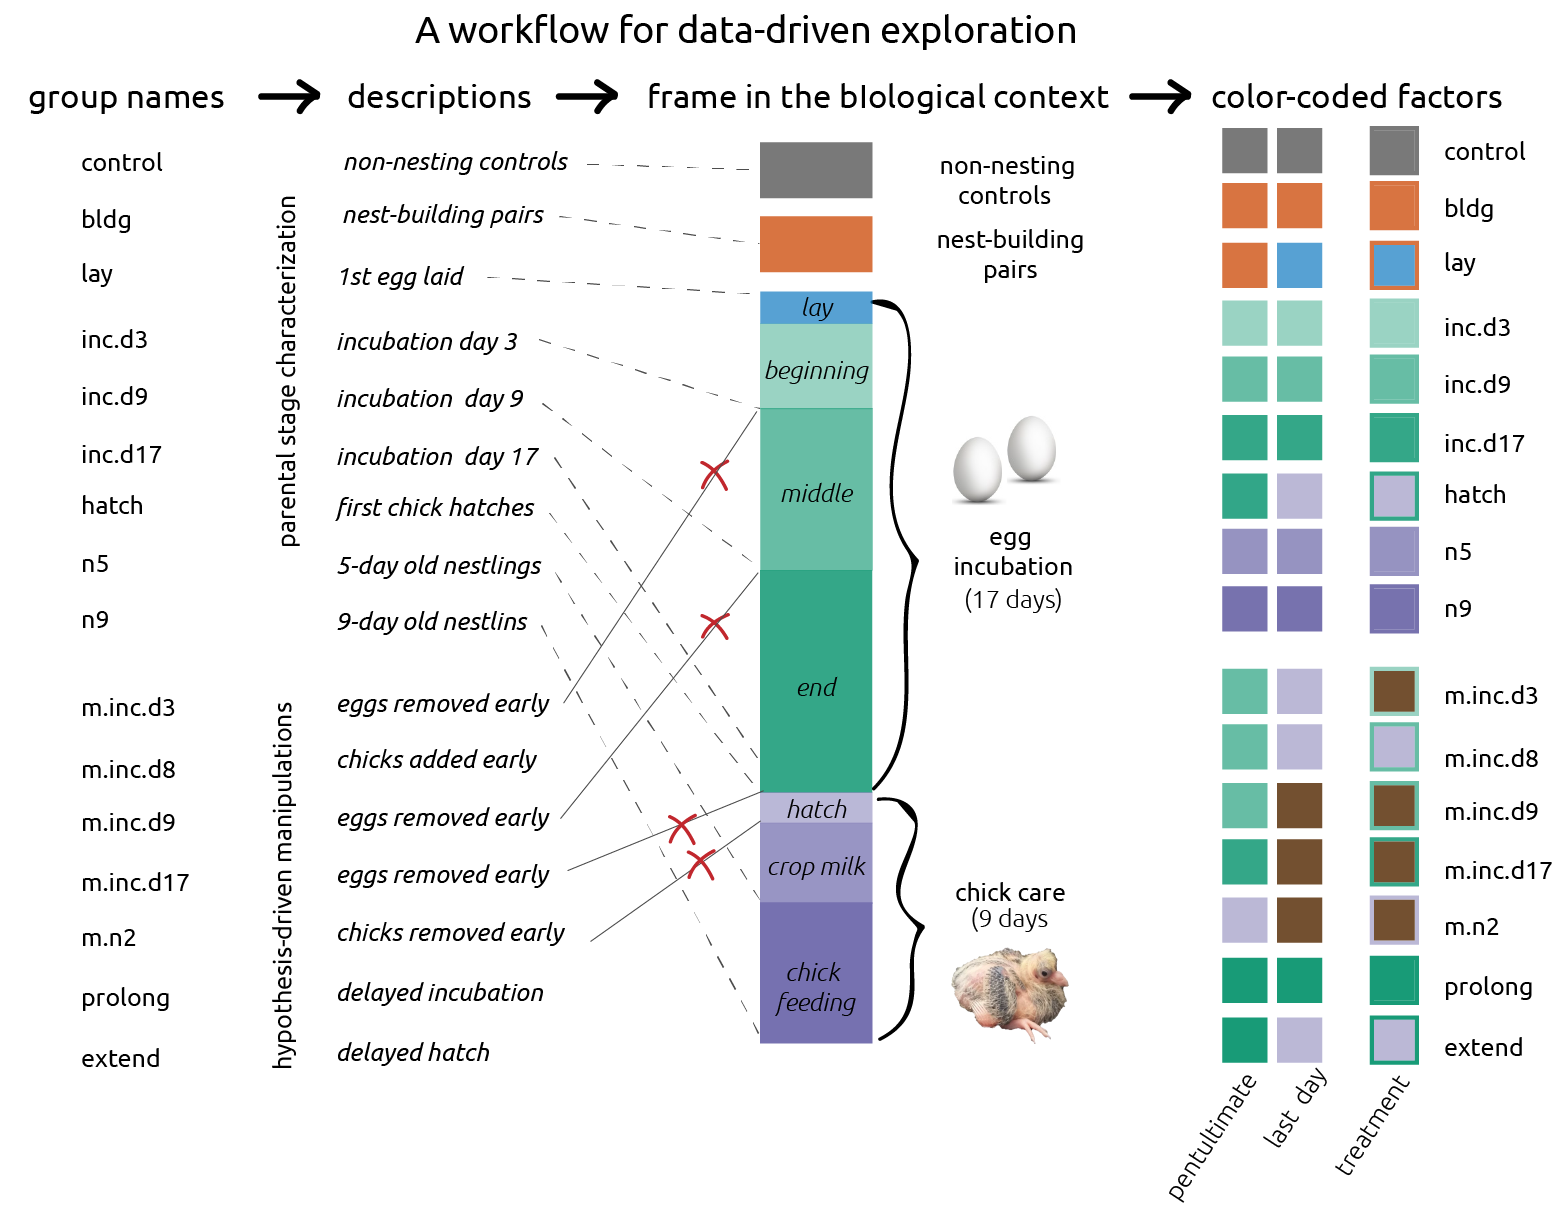
\includegraphics[width=1\linewidth]{DoveParentsRNAseq_design.png}
\end{figure}

Data and analyses are available at \url{https://github.com/macmanes-lab/DoveParentsRNAseq}. For more information visit \url{http://calisilab.ucdavis.edu/}. 

\begin{figure}

\includegraphics[width=0.55\linewidth]{b3.jpg}
\end{figure}


\end{block}


%----------------------------------------------------------------------------------------

\end{column} % End of the first column

\begin{column}{\sepwid}\end{column} % Empty spacer column

\begin{column}{\twocolwid} % Begin a column which is two columns wide (column 2)

\vspace{-0.5em}

\begin{block}{Goal: Minimize hand-typing comparison, maximize reproducibility.} 

\end{block} 


\vspace{-2em}

%----------------------------------------------------------------------------------------

\begin{columns}[t,totalwidth=\twocolwid] % Split up the two columns wide column again

\begin{column}{\onecolwid} % The first column within column 2 (column 2.1)

\vspace{-0.5em}

\begin{block}{{\normalsize New R functions to automate DESeq2}}

\begin{itemize}
  \item \begin{lstlisting} subsetcolData <- function(colData, eachgroup){} \end{lstlisting}
  \item \begin{lstlisting} returntotalDEGs <- function(dds){} \end{lstlisting}
  \item \begin{lstlisting} returnpadj <- function(group1, group2){} \end{lstlisting}
    \item \begin{lstlisting} numDEGs <- function(dds, group1, group2){} \end{lstlisting}
    \item \begin{lstlisting} plottotalDEGs <- function(myDEGS, mysubtitle){} \end{lstlisting}
\end{itemize}

These functions utilize exciting R functions and for loops to compare gene expression across levels.

\begin{figure}
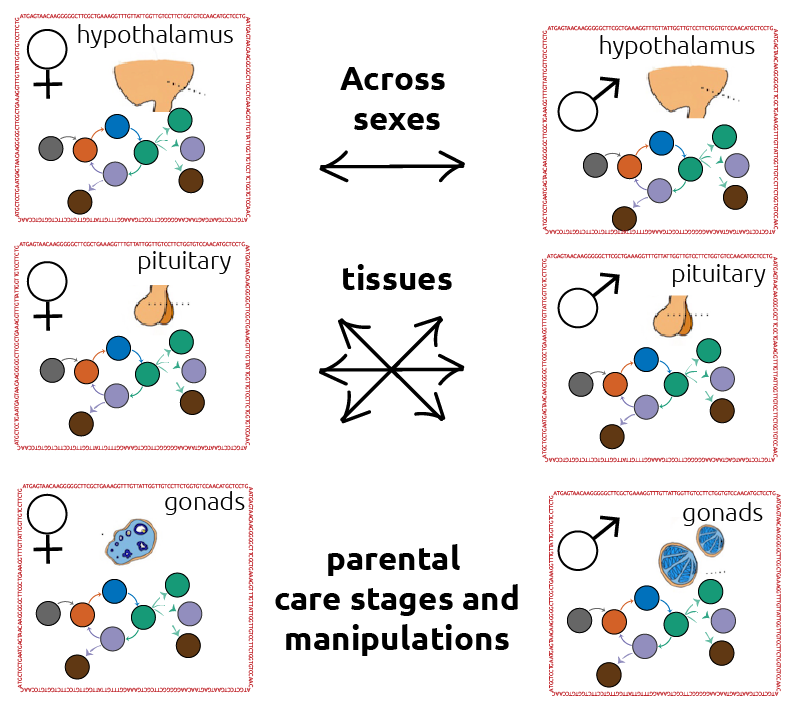
\includegraphics[width=0.75\linewidth]{DoveParentsRNAseq_approach-2.png}
\end{figure}



\end{block}

\begin{block}{{\normalsize Quickly explore variation using the top 500 differentially expressed genes}}

\begin{figure}
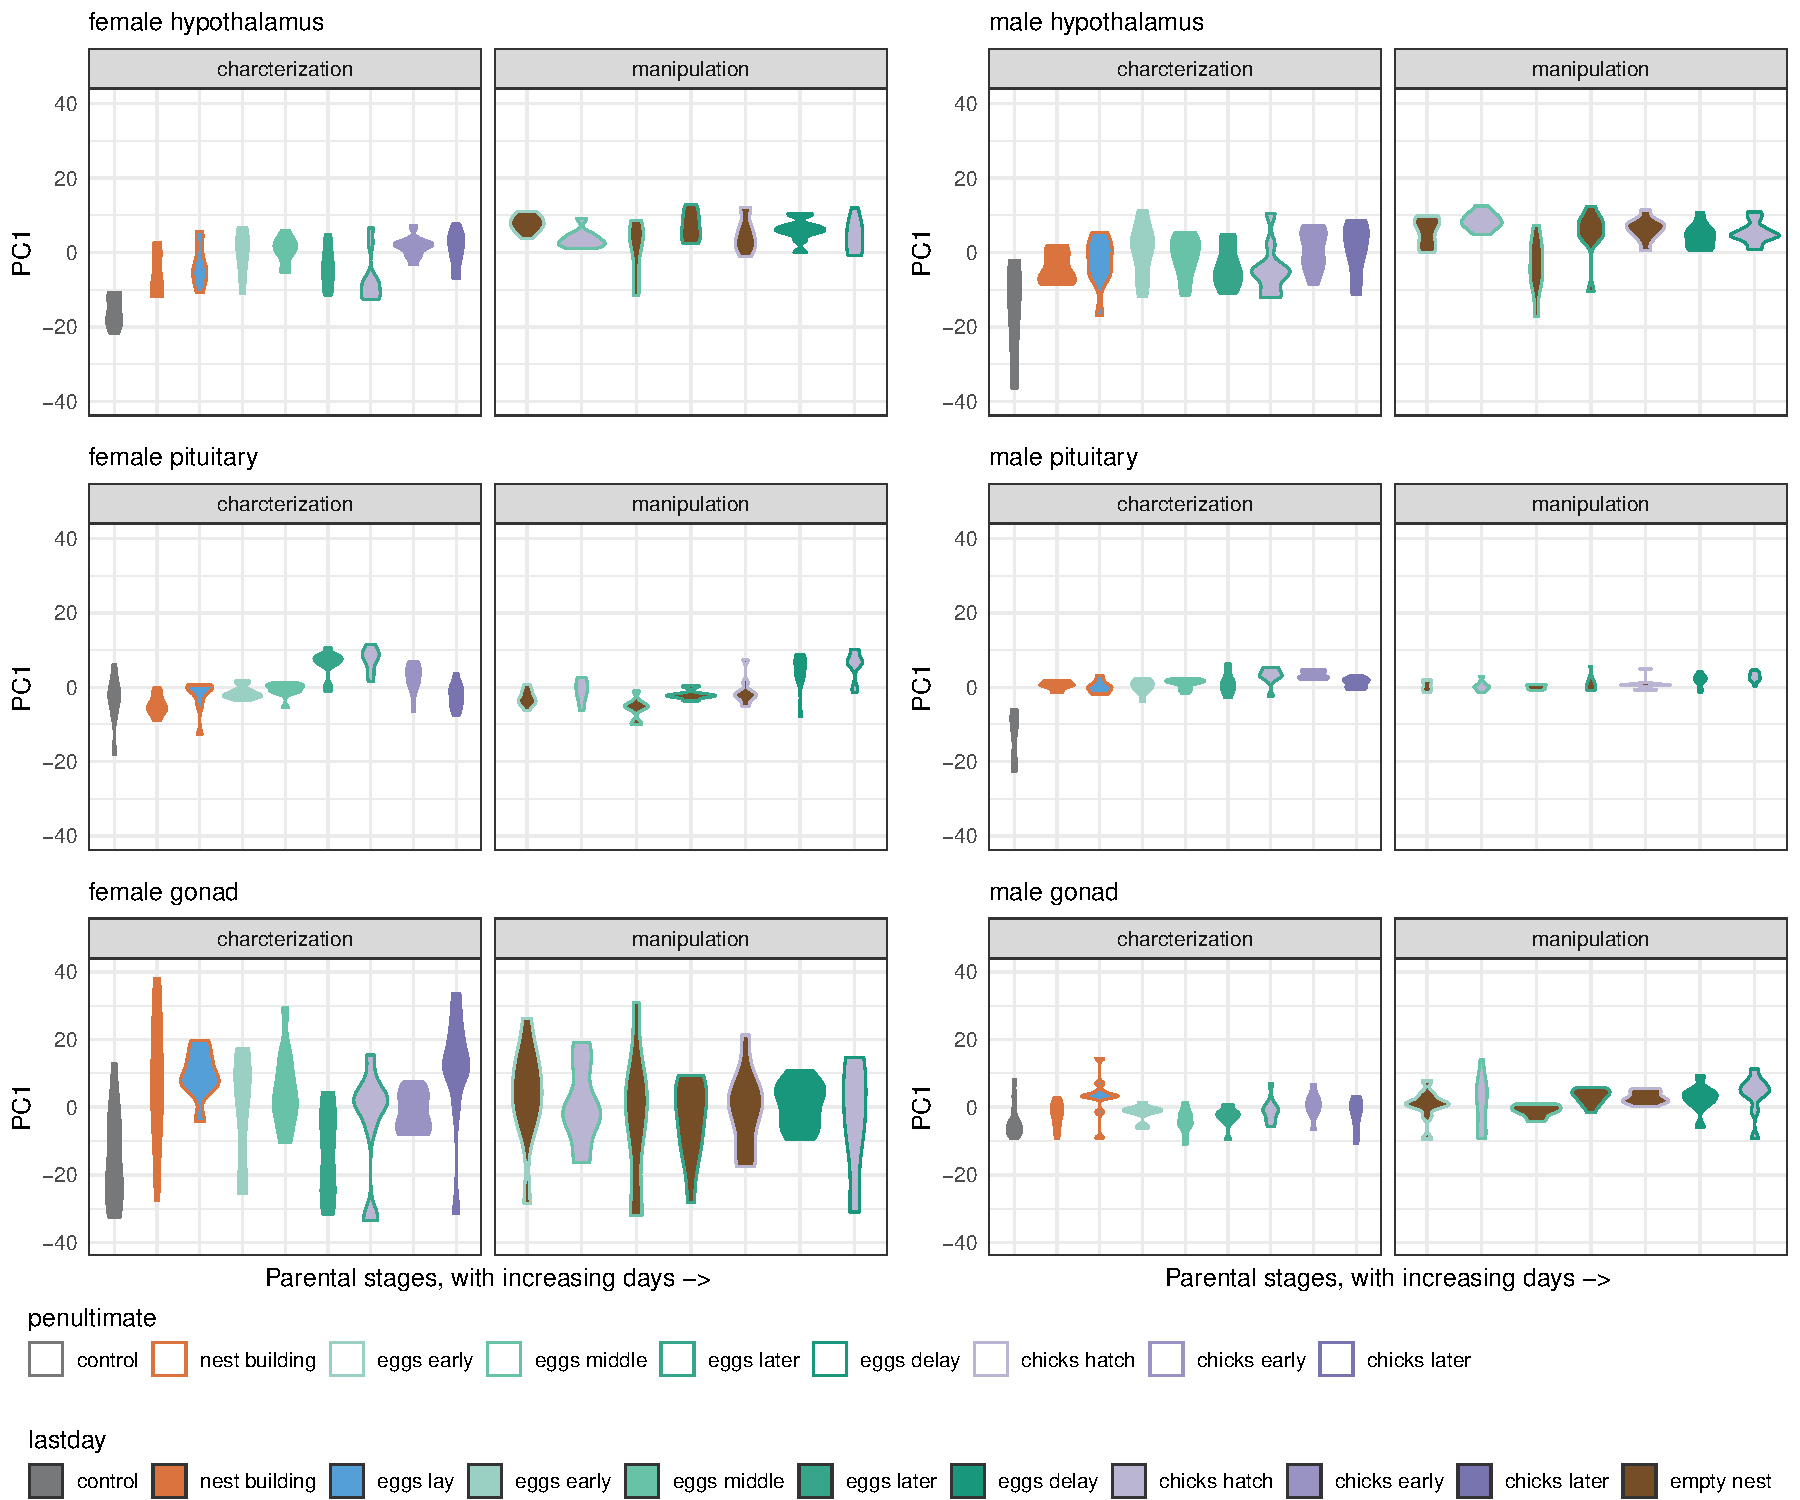
\includegraphics[width=0.9\linewidth]{pca-1.pdf}
\end{figure}


\vspace{0.25em}

\end{block}


 \vspace{-3em}



%----------------------------------------------------------------------------------------

\end{column} % End of column 2.1


\begin{column}{\onecolwid} % The second column within column 2 (column 2.2)

%----------------------------------------------------------------------------------------
%	RESULTS
%----------------------------------------------------------------------------------------

\vspace{-0.5em}

\begin{block}{{\normalsize Calculate and visualize  the total number of differentially expressed genes for each two-way comparison}}

\begin{figure}
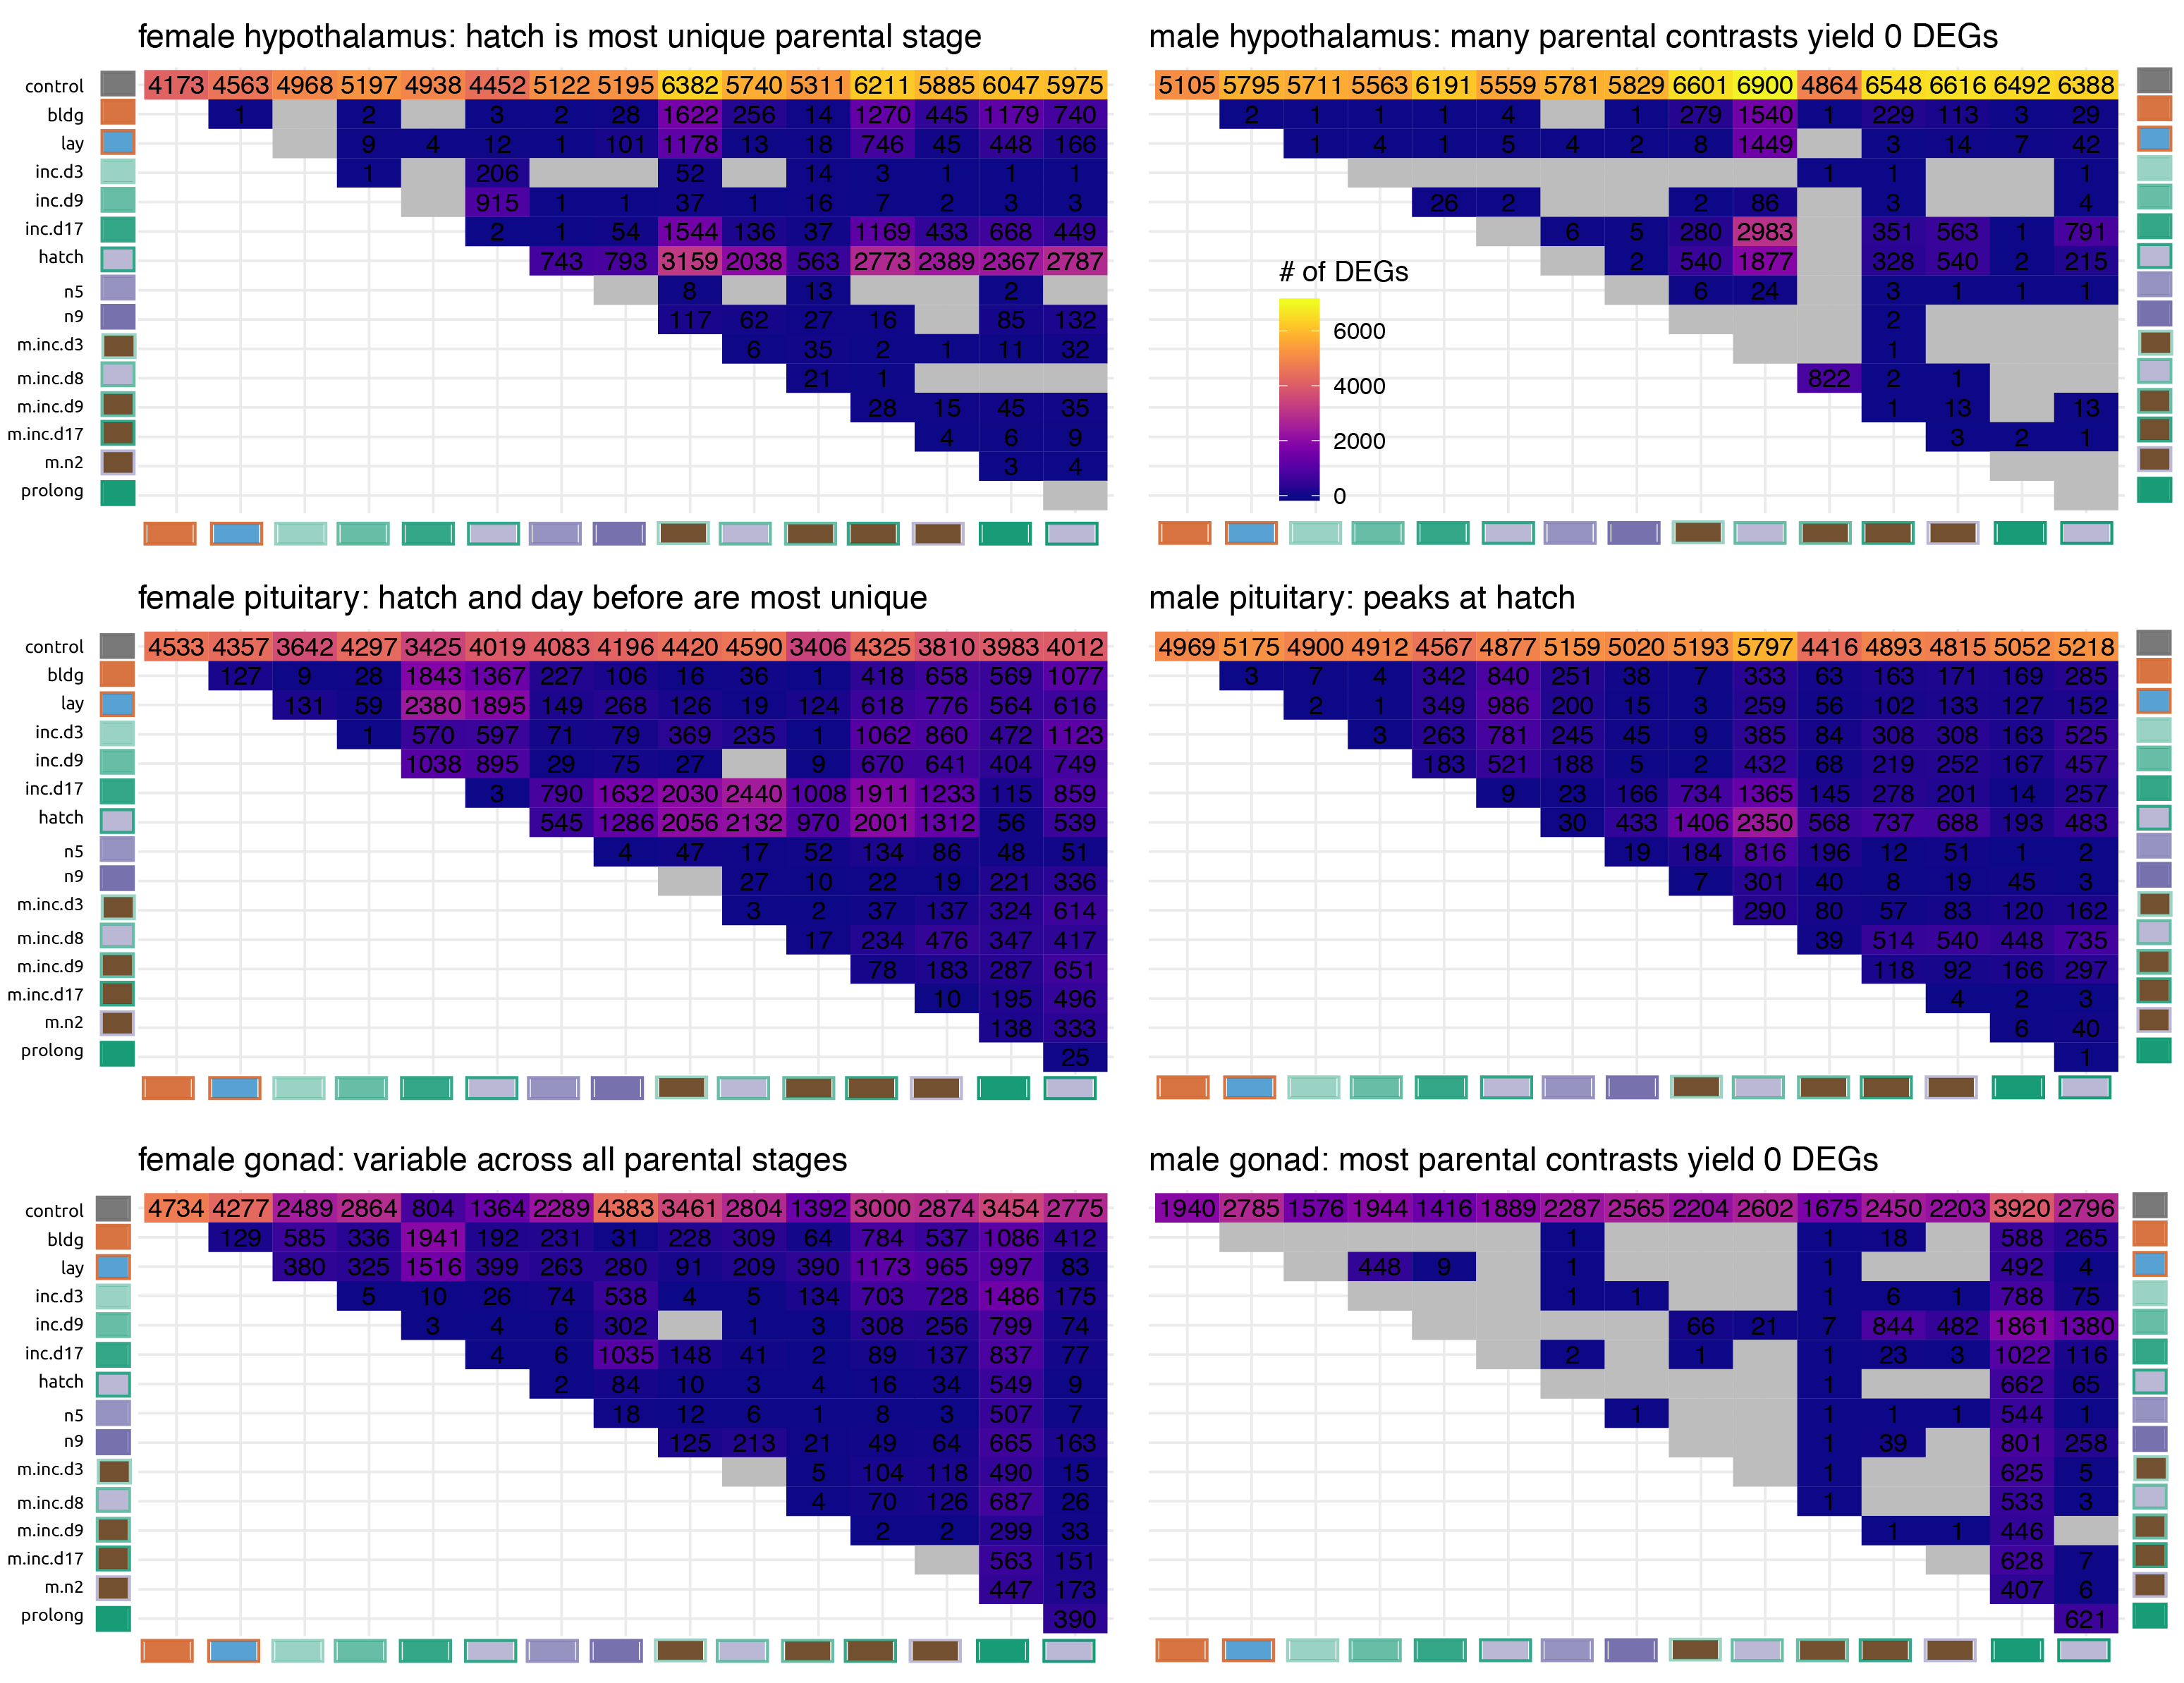
\includegraphics[width=1\linewidth]{DoveParentsRNAseq_totalDEGs.png}
\end{figure}

\end{block}

\begin{block}{{\normalsize Determine the extent of correlation in gene expression variation}}


\begin{figure}
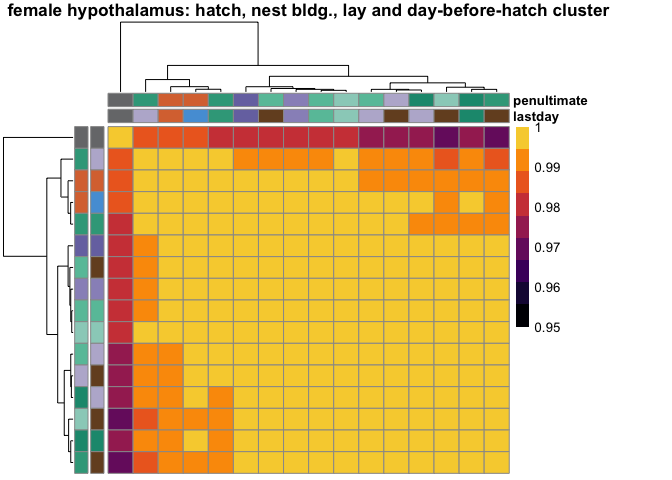
\includegraphics[width=0.5\linewidth]{correlationheatmaps-1.png}
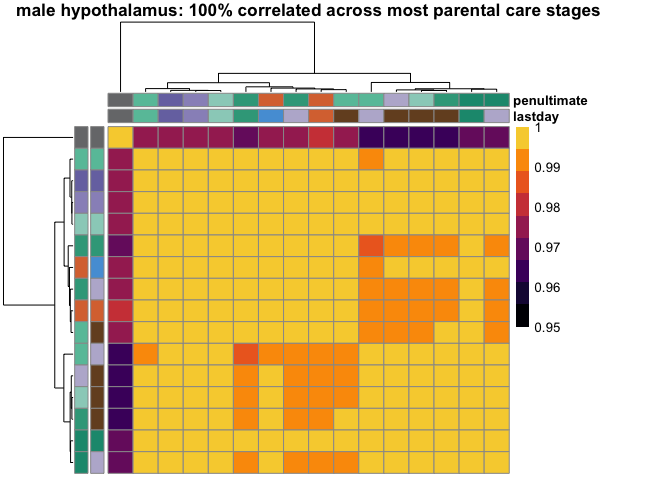
\includegraphics[width=0.5\linewidth]{correlationheatmaps-4.png}
\end{figure}

\begin{figure}
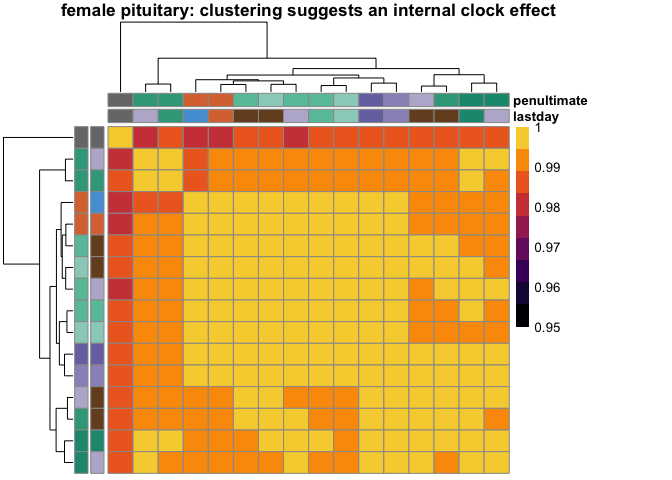
\includegraphics[width=0.5\linewidth]{correlationheatmaps-2.png}
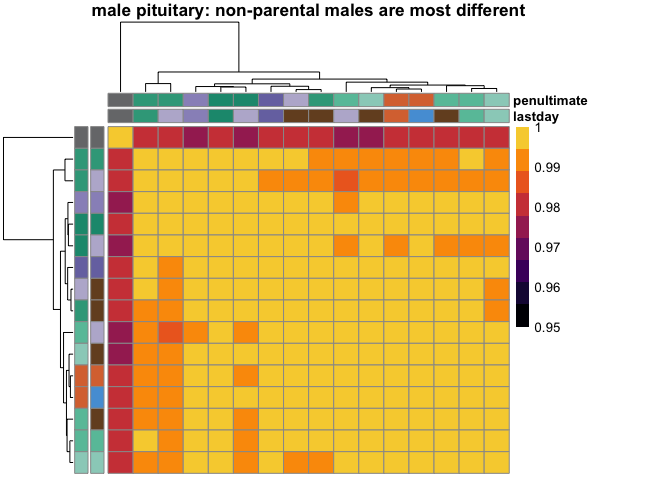
\includegraphics[width=0.5\linewidth]{correlationheatmaps-5.png}
\end{figure}


\begin{figure}
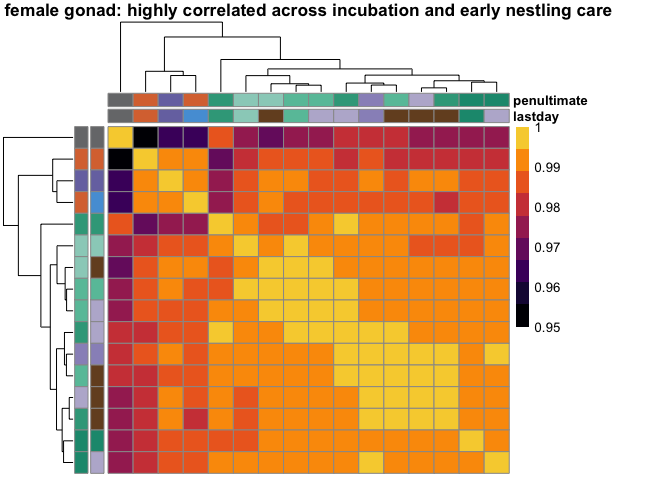
\includegraphics[width=0.5\linewidth]{correlationheatmaps-3.png}
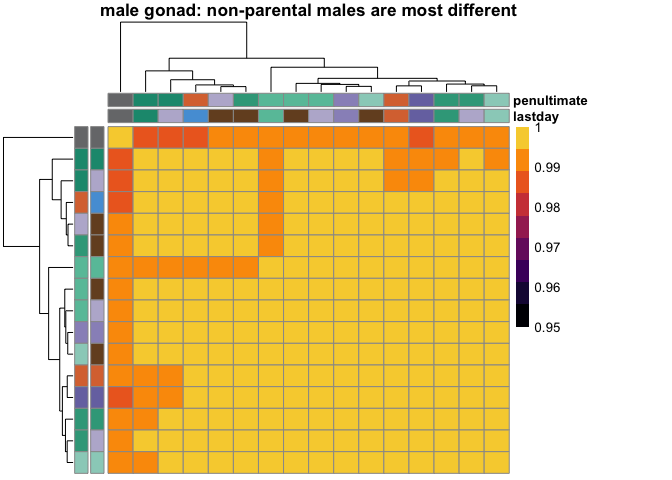
\includegraphics[width=0.5\linewidth]{correlationheatmaps-6.png}
\end{figure}

\end{block}

\vspace{1em}


%----------------------------------------------------------------------------------------

\end{column} % End of column 2.2

\end{columns} % End of the split of column 2

\end{column} % End of the second column

\begin{column}{\sepwid}\end{column} % Empty spacer column

\begin{column}{\onecolwid} % The third column

%----------------------------------------------------------------------------------------
%	panel 4
%----------------------------------------------------------------------------------------

\vspace{-0.5em}

\begin{block}{Preliminary interpretations}

\begin{figure}
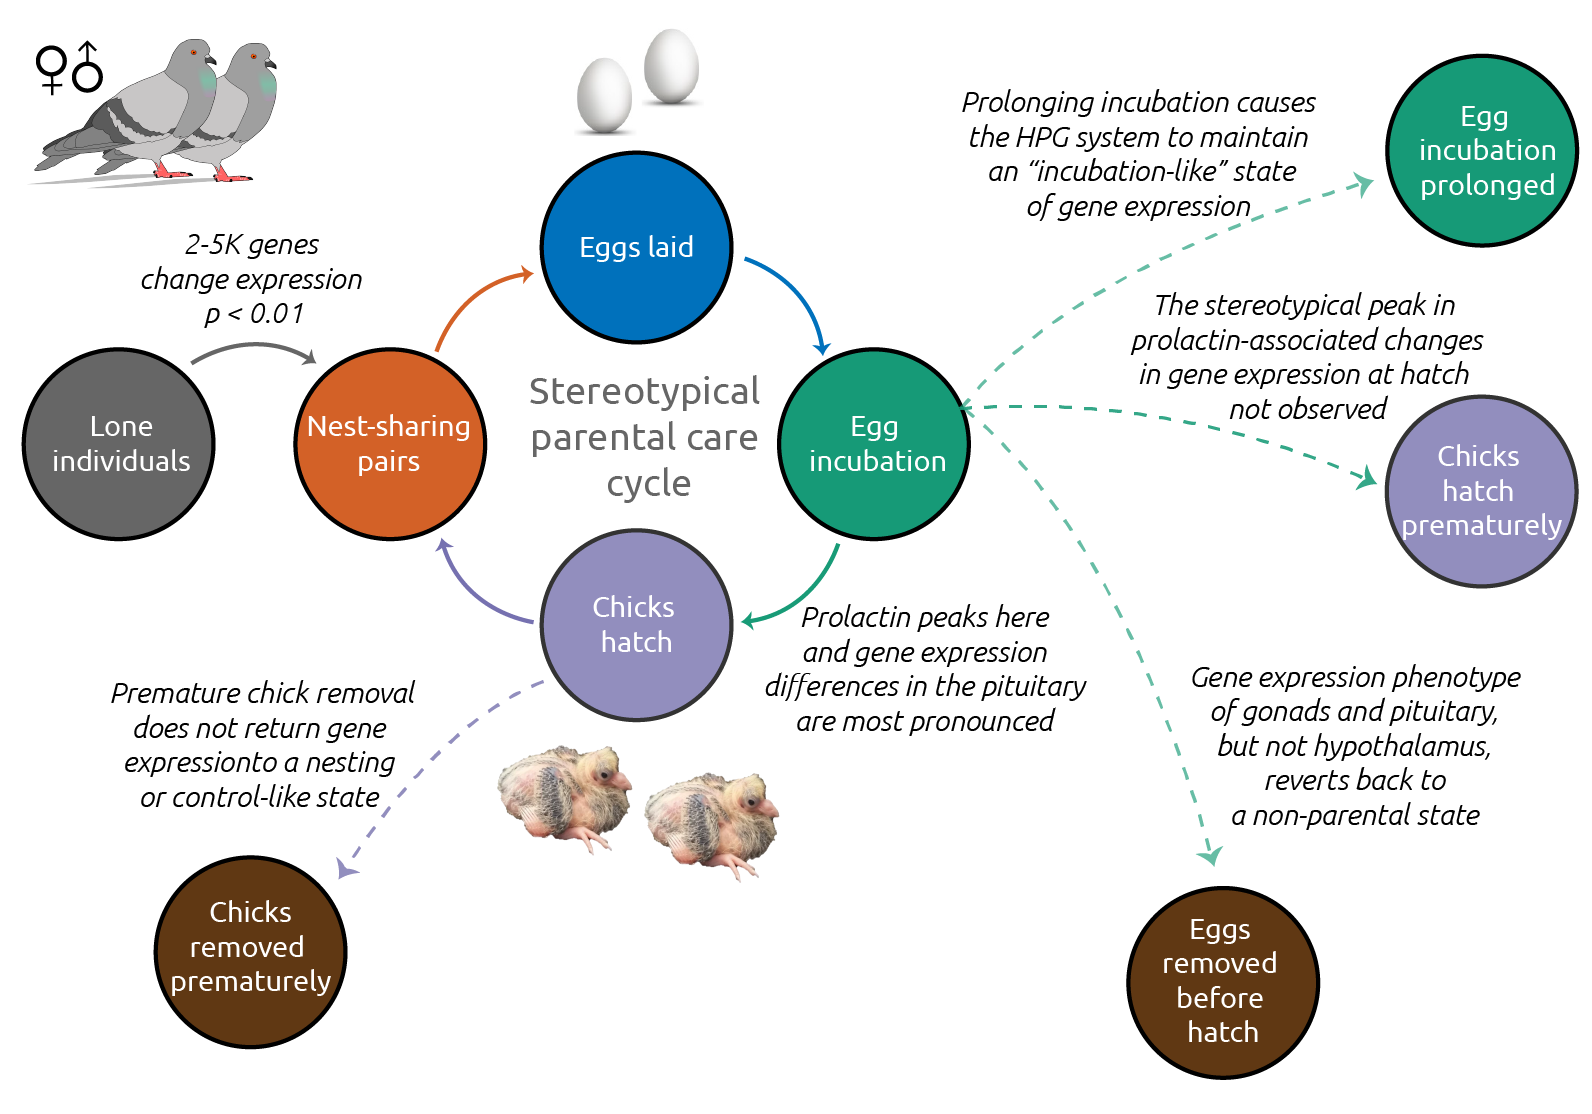
\includegraphics[width=1\linewidth]{DoveParentsRNAseq_summary.png}
%\caption{\url{https://datacarpentry.org/python-ecology-lesson/}}
\end{figure}

\end{block}

\begin{block}{Next steps}

\begin{itemize}
\item \textbf{Zoom out:} examine the full model of sex * tissue * treatment. 
\item \textbf{Zoom in:} examine effects of specific manipulations in greater detail. 
\item \textbf{Test} specific hypotheses. 
\item \textbf{Incorporate} code-review and peer-review . 
\item \textbf{Create} and open source R package. 
\item \textbf{Share} tutorials for how to use the function. 
\end{itemize}

\end{block}

\begin{block}{Acknowledgements}

We are grateful to members of laboratories supervised by RMC, MM, Titus Brown, John Wingfield, Tom Hahn, and Marilyn Ramenofsky for comments and discussion. We thank Victoria Farrar, April Booth, Rechelle Viernes, Jonathan Perez, Jesse Krause, and over 20 undergraduate researchers who helped care for our bird colony. This work is funded by the National Science Foundation, IOS #1455957, to RMC and MM.   

\end{block}


\vspace{0.5em}


\begin{flushright}
\textit{2019-06-15}
\end{flushright}

%----------------------------------------------------------------------------------------

\end{column} % End of the third column

\end{columns} % End of all the columns in the poster

\end{frame} % End of the enclosing frame

\end{document}
